\documentclass{beamer}
\mode<presentation>
\usepackage{amsmath}
\usepackage{amssymb}
%\usepackage{advdate}
\usepackage{adjustbox}
\usepackage{subcaption}
\usepackage{enumitem}
\usepackage{multicol}
\usepackage{mathtools}
\usepackage{listings}
\usepackage{url}
\def\UrlBreaks{\do\/\do-}
\usetheme{Boadilla}
\usecolortheme{lily}
\setbeamertemplate{footline}
{
  \leavevmode%
  \hbox{%
  \begin{beamercolorbox}[wd=\paperwidth,ht=2.25ex,dp=1ex,right]{author in head/foot}%
    \insertframenumber{} / \inserttotalframenumber\hspace*{2ex} 
  \end{beamercolorbox}}%
  \vskip0pt%
}
\setbeamertemplate{navigation symbols}{}

\providecommand{\nCr}[2]{\,^{#1}C_{#2}} % nCr
\providecommand{\nPr}[2]{\,^{#1}P_{#2}} % nPr
\providecommand{\mbf}{\mathbf}
\providecommand{\pr}[1]{\ensuremath{\Pr\left(#1\right)}}
\providecommand{\qfunc}[1]{\ensuremath{Q\left(#1\right)}}
\providecommand{\sbrak}[1]{\ensuremath{{}\left[#1\right]}}
\providecommand{\lsbrak}[1]{\ensuremath{{}\left[#1\right.}}
\providecommand{\rsbrak}[1]{\ensuremath{{}\left.#1\right]}}
\providecommand{\brak}[1]{\ensuremath{\left(#1\right)}}
\providecommand{\lbrak}[1]{\ensuremath{\left(#1\right.}}
\providecommand{\rbrak}[1]{\ensuremath{\left.#1\right)}}
\providecommand{\cbrak}[1]{\ensuremath{\left\{#1\right\}}}
\providecommand{\lcbrak}[1]{\ensuremath{\left\{#1\right.}}
\providecommand{\rcbrak}[1]{\ensuremath{\left.#1\right\}}}
\theoremstyle{remark}
\newtheorem{rem}{Remark}
\newcommand{\sgn}{\mathop{\mathrm{sgn}}}
\providecommand{\abs}[1]{\left\vert#1\right\vert}
\providecommand{\res}[1]{\Res\displaylimits_{#1}} 
\providecommand{\norm}[1]{\lVert#1\rVert}
\providecommand{\mtx}[1]{\mathbf{#1}}
\providecommand{\mean}[1]{E\left[ #1 \right]}
\providecommand{\fourier}{\overset{\mathcal{F}}{ \rightleftharpoons}}
%\providecommand{\hilbert}{\overset{\mathcal{H}}{ \rightleftharpoons}}
\providecommand{\system}{\overset{\mathcal{H}}{ \longleftrightarrow}}
	%\newcommand{\solution}[2]{\textbf{Solution:}{#1}}
%\newcommand{\solution}{\noindent \textbf{Solution: }}
\providecommand{\dec}[2]{\ensuremath{\overset{#1}{\underset{#2}{\gtrless}}}}
\newcommand{\myvec}[1]{\ensuremath{\begin{pmatrix}#1\end{pmatrix}}}
\newcommand{\mydet}[1]{\ensuremath{\begin{vmatrix}#1\end{vmatrix}}}
\let\vec\mathbf

\lstset{
%language=C,
frame=single, 
breaklines=true,
columns=fullflexible
}

\numberwithin{equation}{section}

\title{4.13.61}
\author{Rushil Shanmukha Srinivas \\EE25BTECH11057 \\ Electrical Enggineering ,\\IIT Hyderabad.}

\date{\today} 
\begin{document} 

\begin{frame}
\titlepage
\end{frame}

\section*{Outline}
\begin{frame}
\tableofcontents
\end{frame}
\section{Problem}
\begin{frame}
\frametitle{Problem Statement}
\textbf{Question} : 
A rectangle $PQRS$ has its side $\vec{P}\vec{Q}$ parallel to the line $y = mx$ and vertices $\vec{P}, \vec{Q} \ and \ \vec{S}$ on the lines $y = a, x = b \ and \ x = -b $ ,respectively. Find the locus of the vertex $\vec{R}$.


\end{frame}
\section{Solution}
\subsection{ Dot Product  and Locus}
\begin{frame}
\frametitle{Dot Product and Locus}
%\framesubtitle{Literature}
\textbf{Solution:}

\begin{align}
y=mx \Longrightarrow \vec{n}^\top\vec{x}=0,\vec{n}=\myvec{-m\\1}
\end{align}
The equation of $\vec{P}\vec{Q}$ is $\vec{n}^\top\vec{x}=c$

Let 
\begin{align}
\vec{P}=\myvec{x_1\\a},\vec{Q}=\myvec{b\\y_1},\vec{R}=\myvec{X\\Y},\vec{S}=\myvec{-b\\y_2}
\end{align}
In rectangle diagonals bisect each other
\begin{align}
\vec{P}+\vec{R}=\vec{Q}+\vec{S} \Longrightarrow \myvec{x_1+X\\a+Y}=\myvec{0\\y_1+y_2} 
\end{align}
\begin{align}
x_1=-X, a+Y=y_1+y_2
\end{align}
\begin{align}
\vec{n}^\top\vec{P}=\vec{n}^\top\vec{Q}=c \Longrightarrow \myvec{-m & 1}\myvec{-X\\a}=\myvec{-m & 1}\myvec{b\\y_1}
\end{align}
\end{frame}
\begin{frame}
\begin{align}
mX+a = -mb+y_1 \Longrightarrow m(X+b)+a=a+Y-y_2
\end{align}
\begin{align}
m(X+b)+y_2 = Y
\end{align}
\begin{align}
\vec{Q}-\vec{P}=\myvec{b+X\\y_1-a},\vec{S}-\vec{P}=\myvec{X-b\\y_2-a}
\end{align}
In  rectangle  PQRS,
\begin{align}
 \vec{P}\vec{Q} \perp \vec{P}\vec{S} \Longrightarrow (\vec{Q}-\vec{P})^\top(\vec{S}-\vec{P})=0 
\end{align}
\begin{align}
\myvec{b+X & Y-y_2}\myvec{X-b\\y_2-a} = 0 
\end{align}
\begin{align}
\myvec{b+X & m(X+b)}\myvec{X-b\\Y-m(X+b)-a} = 0
\end{align}
\begin{align}
(X+b)(X-b+mY-m^2(X+b)-ma) = 0
\end{align}
\begin{align}
X+b = 0 \ or \ (1-m^2)X+mY-(b(1+m^2)+am) = 0
\end{align}
\end{frame}
\begin{frame}
X+b = 0  is not locus of vertex $\vec{R}$ as it gives a fixed point.

The locus is
\begin{align}
(1-m^2)X+mY-(b(1+m^2)+am) = 0
\end{align}

\end{frame}

\subsection{Plots}
\begin{frame}
\frametitle{Plots}
\begin{figure}
\centering
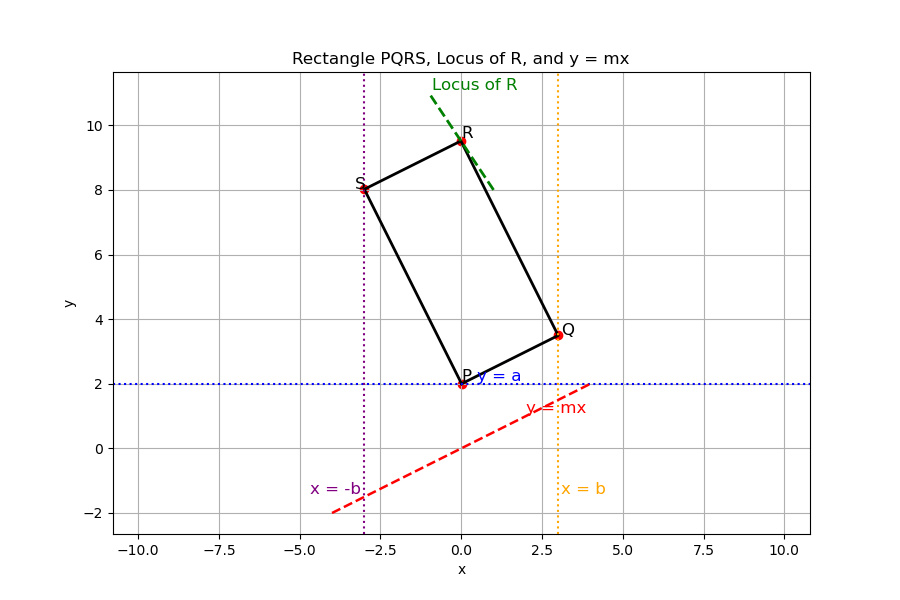
\includegraphics[width=0.9\columnwidth]{figs/locus.png}
\caption{fig : Representation of Rectangle and Locus}
\label{Fig9}
\end{figure}
\end{frame}
\section{C Code}
\begin{frame}[fragile]
\frametitle{C Code }
\begin{lstlisting}[language=C]  
   #include <stdio.h>
/*
   A rectangle PQRS has its side PQ parallel to the line y = mx
   and vertices P, Q, S on lines y=a, x=b, x=-b respectively.
   Find the locus of vertex R.
   Result: y = m*x - (a*(1+m^2))/m,  with x = ±b
*/

double find_locus(double m, double a, double x) {
    return m * x - (a * (1 + m * m)) / m;}

int main() {
    double m, a, b;

    printf("Enter slope m: ");
    scanf("%lf", &m);
    \end{lstlisting}
    \end{frame}
    \begin{frame}[fragile]
    \begin{lstlisting}

    printf("Enter constant a (line y=a): ");
    scanf("%lf", &a);

    printf("Enter constant b (lines x=±b): ");
    scanf("%lf", &b);

    // For x = +b
    double y1 = find_locus(m, a, b);
    printf("For x = %.2f, R = (%.2f, %.2f)\n", b, b, y1);

    // For x = -b
    double y2 = find_locus(m, a, -b);
    printf("For x = %.2f, R = (%.2f, %.2f)\n", -b, -b, y2);

    return 0;
}


\end{lstlisting}
\end{frame}

\section{Python Code}
\begin{frame}[fragile]
\frametitle{Python : call\_c.py}
\begin{lstlisting}
import ctypes

# Load the compiled shared object
# Make sure rectangle_locus.so is in the same directory
lib = ctypes.CDLL('./rectangle_locus.so')
# Define the argument and return types of the C function
# double find_locus(double m, double a, double x)
lib.find_locus.argtypes = [ctypes.c_double, ctypes.c_double, ctypes.c_double]
lib.find_locus.restype = ctypes.c_double

def call_find_locus(m, a, b):
    results = [ ]
    for x in [b, -b]:
        y = lib.find_locus(m, a, x)
        results.append((x, y))
    return results
\end{lstlisting}
\end{frame}
\begin{frame}[fragile]
\begin{lstlisting}
if __name__ == "__main__":
    # Example values (you can change these)
    m, a, b = 2.0, 3.0, 4.0

    points = call_find_locus(m, a, b)
    for x, y in points:
        print(f"R = ({x:.2f}, {y:.2f})")

\end{lstlisting}
\end{frame}

\begin{frame}[fragile]
\frametitle{Python Code for Plotting}
\begin{lstlisting}[language=Python]

import numpy as np
import matplotlib.pyplot as plt

# Parameters
m = 0.5      # slope of PQ and the reference line y = mx
a = 2        # y = a
b = 3        # x = b
x_P = np.linspace(-1, 1, 100)  # vary x-coordinate of P

# Coordinates of Q, S, R
y_Q = m*(b - x_P) + a
y_S = a + (b + x_P)/m
x_R = -x_P
y_R = y_Q + y_S - a

# Pick an example rectangle
\end{lstlisting}
\end{frame}
\begin{frame}[fragile]
\begin{lstlisting}
example_idx = 50
P = (x_P[example_idx], a)
Q = (b, y_Q[example_idx])
S = (-b, y_S[example_idx])
R = (x_R[example_idx], y_R[example_idx])

# Rectangle vertices order for plotting
rect_x = [P[0], Q[0], R[0], S[0], P[0]]
rect_y = [P[1], Q[1], R[1], S[1], P[1]]
plt.figure(figsize=(9,6))
# Plot rectangle
plt.plot(rect_x, rect_y, 'k-', linewidth=2)
plt.scatter([P[0], Q[0], R[0], S[0]], [P[1], Q[1], R[1], S[1]], color='red')

# Plot locus of R
plt.plot(x_R, y_R, 'g--', linewidth=2)
plt.text(x_R[-1]+0.1, y_R[-1], 'Locus of R', color='green', fontsize=12, verticalalignment='bottom')
\end{lstlisting}
\end{frame}
\begin{frame}[fragile]
\begin{lstlisting}
# Constraint lines and labels
plt.axhline(a, color='blue', linestyle=':', linewidth=1.5)
plt.text(0.5, a+0.1, 'y = a', color='blue', fontsize=12)

plt.axvline(b, color='orange', linestyle=':', linewidth=1.5)
plt.text(b+0.1, -1.5, 'x = b', color='orange', fontsize=12, verticalalignment='bottom')

plt.axvline(-b, color='purple', linestyle=':', linewidth=1.5)
plt.text(-b-0.1, -1.5, 'x = -b', color='purple', fontsize=12, horizontalalignment='right', verticalalignment='bottom')

# Plot y = mx line passing through origin
x_line = np.linspace(-4, 4, 100)
y_line = m * x_line
plt.plot(x_line, y_line, 'r--', linewidth=1.8)
plt.text(2, m*2+0.1, 'y = mx', color='red', fontsize=12)
\end{lstlisting}
\end{frame}
\begin{frame}[fragile]
\begin{lstlisting}
# Label rectangle vertices
plt.text(P[0], P[1]+0.1, 'P', fontsize=12)
plt.text(Q[0]+0.1, Q[1], 'Q', fontsize=12)
plt.text(R[0], R[1]+0.1, 'R', fontsize=12)
plt.text(S[0]-0.3, S[1], 'S', fontsize=12)

# Set limits to see full rectangle and lines
plt.xlim(-4, 4)
plt.ylim(min(min(y_R), -2), max(max(y_R), 4))

plt.xlabel('x')
plt.ylabel('y')
plt.title('Rectangle PQRS, Locus of R, and y = mx')
plt.grid(True)
plt.axis('equal')
plt.savefig("../figs/locus.png")
plt.show()


\end{lstlisting}
\end{frame}

\end{document}
  